\documentclass[UTF8,zihao=-4,openany,fontset=none]{ctexrep}

\usepackage[a4paper,top=2.5cm,bottom=2.5cm,left=2.7cm,right=2.7cm]{geometry}
\usepackage{fontspec}
\usepackage{xeCJK}
\usepackage{graphicx}
\usepackage{booktabs}
\usepackage{tabularx}
\usepackage{longtable}
\usepackage{array}
\usepackage{listings}
\usepackage{xcolor}
\usepackage{xurl}
\usepackage{hyperref}
\usepackage{bookmark}
\usepackage{caption}
\usepackage{float}
\usepackage{enumitem}
\usepackage[most]{tcolorbox}
\usepackage{tikz}
\usetikzlibrary{arrows.meta,positioning,shapes.geometric}
\usepackage{fancyhdr}
\usepackage{lastpage}
\usepackage{setspace}
\usepackage{needspace}

\setmainfont{TeX Gyre Termes}
\setsansfont{TeX Gyre Heros}
\setmonofont[
  BoldFont=texgyrecursor-bold.otf,
  ItalicFont=texgyrecursor-italic.otf
]{texgyrecursor-regular.otf}
\setCJKmainfont[
  BoldFont=FandolSong-Bold.otf,
  ItalicFont=FandolKai-Regular.otf
]{FandolSong-Regular.otf}
\setCJKsansfont[
  BoldFont=FandolHei-Bold.otf
]{FandolHei-Regular.otf}
\setCJKmonofont{FandolFang-Regular.otf}
\setlength{\emergencystretch}{3em}

\definecolor{osblue}{HTML}{164E63}
\definecolor{oscyan}{HTML}{0891B2}
\definecolor{oslight}{HTML}{ECFEFF}
\definecolor{osgray}{HTML}{475569}
\definecolor{codebg}{HTML}{F8FAFC}
\definecolor{codeframe}{HTML}{CBD5E1}

\hypersetup{
  colorlinks=true,
  linkcolor=osblue,
  urlcolor=oscyan,
  citecolor=osblue,
  pdftitle={Linux 启动初始化过程探析},
  pdfauthor={XXX}
}

\pagestyle{fancy}
\setlength{\headheight}{15pt}
\fancyhf{}
\fancyhead[L]{操作系统实验三}
\fancyhead[R]{Linux 启动初始化过程探析}
\fancyfoot[C]{第 \thepage\ 页，共 \pageref{LastPage} 页}
\renewcommand{\headrulewidth}{0.4pt}
\fancypagestyle{plain}{
\fancyhf{}
\fancyhead[L]{操作系统实验三}
\fancyhead[R]{Linux 启动初始化过程探析}
\fancyfoot[C]{第 \thepage\ 页，共 \pageref{LastPage} 页}
\renewcommand{\headrulewidth}{0.4pt}
}

\ctexset{
  chapter={format=\LARGE\bfseries\color{osblue},number=\chinese{chapter},beforeskip=12pt,afterskip=18pt},
  section={format=\Large\bfseries\color{osblue}},
  subsection={format=\large\bfseries\color{osgray}}
}

\lstset{
  basicstyle=\small\ttfamily,
  backgroundcolor=\color{codebg},
  frame=single,
  rulecolor=\color{codeframe},
  numbers=left,
  numberstyle=\scriptsize\color{osgray},
  breaklines=true,
  breakatwhitespace=false,
  columns=fullflexible,
  keepspaces=true,
  showstringspaces=false,
  keywordstyle=\color{osblue}\bfseries,
  commentstyle=\color{osgray},
  stringstyle=\color{oscyan},
  xleftmargin=1.5em,
  framexleftmargin=1em
}

\newcommand{\placeholder}[1]{\texttt{#1}}
\newcommand{\kernelver}{6.12.110-oslab3-xxx}
\newcommand{\sourcever}{6.12.110}
\newcommand{\oldkernel}{6.11.0-26-kfocus}
\newcommand{\buildelapsed}{1 小时 12 分 32 秒（成功重编译；首轮失败用时 43 分 26 秒）}

\newcommand{\evidencefigure}[4][0.96\textwidth]{%
  \begin{figure}[H]
    \centering
    \IfFileExists{#2}{\includegraphics[width=#1]{#2}}{%
      \fbox{\parbox[c][5cm][c]{0.9\textwidth}{\centering #4}}}
    \caption{#3}
  \end{figure}
}

\newtcolorbox{resultbox}[1]{
  colback=oslight,
  colframe=oscyan,
  fonttitle=\bfseries,
  title=#1,
  arc=2mm,
  boxrule=0.7pt
}

\begin{document}

\begin{titlepage}
  \centering
  \vspace*{1.5cm}
  {\Large 北京交通大学计算机学院\par}
  \vspace{1.2cm}
  {\color{osblue}\rule{0.9\textwidth}{1.2pt}\par}
  \vspace{1.1cm}
  {\Huge\bfseries 操作系统实验报告\par}
  \vspace{0.7cm}
  {\LARGE 实验三：Linux 启动初始化过程探析\par}
  \vspace{1.1cm}
  {\color{osblue}\rule{0.9\textwidth}{1.2pt}\par}
  \vfill
  \renewcommand{\arraystretch}{1.7}
  \begin{tabular}{>{\bfseries}r l}
    姓名：& XXX \\
    学号：& XXX \\
    班级：& XXX \\
    指导教师：& XXX \\
    实验平台：& VMware Workstation + Kubuntu 24.04.3 LTS \\
    实验日期：& 2026 年 9 月 21 日 \\
  \end{tabular}
  \vfill
  {\large 个人信息暂以 XXX 占位\par}
\end{titlepage}

\chapter*{摘要}
\addcontentsline{toc}{chapter}{摘要}
本实验以 VMware Workstation 中的 Kubuntu 24.04.3 LTS 虚拟机为平台，下载并研读 Linux
\sourcever 长期维护内核源码，围绕 x86\_64 体系结构梳理从 BIOS、GRUB、实模式引导代码、
保护模式与长模式入口，到体系结构无关的 \texttt{start\_kernel()}、\texttt{rest\_init()}、
\texttt{kernel\_init()} 以及 systemd 用户空间初始化的完整路径。在保留原内核的前提下，
基于当前配置生成适合该虚拟机硬件的裁剪配置，编译并安装带有唯一后缀的
\kernelver 内核，最后通过运行版本、内核日志、SSH 网络连通性及系统服务状态进行验证。
实验过程保留源码定位、配置、编译、安装与启动证据，形成可复现的命令和日志链。
额外实现一个可加载的内核探针，通过 procfs 与内核日志观察模块初始化，并在实际重启后完成九项检查。
基础运行数据采集于 2026 年 9 月 21 日；10 月 5 日首次发布，10 月 7 日补充文档和交互证据，
并在虚拟机内完成九项复验与六项补充检查，均通过。个人字段保留 XXX，现附带个人标题的真实对话截图。

\textbf{关键词：} Linux 内核；x86\_64；启动初始化；start\_kernel；GRUB；内核编译

\tableofcontents

\chapter{实验目的与要求}

\section{实验目的}
\begin{enumerate}[label=(\arabic*)]
  \item 理解操作系统从固件引导到用户空间初始化的分阶段机制；
  \item 识别 x86\_64 处理器相关代码与体系结构无关初始化代码的边界；
  \item 掌握 Linux 内核源码的配置、编译、安装、引导和验证方法；
  \item 建立“源码调用路径—启动日志—运行结果”三者之间的一致性证据。
\end{enumerate}

\section{任务与证据映射}
本报告按实验指导的内容要求组织\cite{guide}。
\begin{table}[H]
  \centering
  \caption{实验要求与本文证据的对应关系}
  \begin{tabularx}{\textwidth}{p{0.20\textwidth}p{0.16\textwidth}X}
    \toprule
    实验要求 & 对应章节 & 主要证据 \\
    \midrule
    下载和研读内核源码 & 第 3、4 章 & kernel.org 发布信息、SHA-256、源码文件与行号 \\
    分析启动初始化机理 & 第 3、4 章 & 分阶段流程图、关键入口、处理器相关/无关部分划分 \\
    编译并启用内核 & 第 5、6 章 & 配置、编译日志、内核产物、GRUB 和新内核运行结果 \\
    一致性检查 & 第 7 章 & \texttt{uname}、\texttt{journalctl -b -k} 与源码对照 \\
    Agent 协作与过程证据 & 第 10 章 & 运行截图、个人标题对话截图与文字节选 \\
    \bottomrule
  \end{tabularx}
\end{table}

\chapter{实验环境}

\section{软硬件环境}
\begin{table}[H]
  \centering
  \caption{实验环境信息}
  \begin{tabularx}{\textwidth}{p{0.27\textwidth}X}
    \toprule
    项目 & 配置 \\
    \midrule
    虚拟化平台 & VMware Workstation，虚拟硬件版本 21，NAT 网络 \\
    客户机系统 & Ubuntu/Kubuntu 24.04.3 LTS，x86\_64 \\
    处理器与内存 & 2 个虚拟 CPU，系统可见总内存 3.8 GiB，511 MiB Swap \\
    存储 & 根分区 196 GiB（实验开始时约 185 GiB 可用）；\texttt{/boot} 4.0 GiB \\
    原始内核 & \oldkernel \\
    目标内核 & \kernelver \\
    编译器 & GCC 13.3.0，GNU Make 4.3 \\
    远程操作 & OpenSSH，地址 \texttt{192.168.81.128}，Ed25519 公钥认证 \\
    报告工具 & XeLaTeX（TeX Live 2026）、Poppler \\
    \bottomrule
  \end{tabularx}
\end{table}

\section{远程操作与证据策略}
为降低长时间编译过程中桌面操作的干扰，先配置 Windows 主机到虚拟机的 SSH 公钥认证。
公钥仅追加到 \texttt{\textasciitilde/.ssh/authorized\_keys}，保留密码认证作为回退。
终端证据由 Kubuntu 桌面会话中的 Konsole 实际执行命令后，通过 Spectacle 捕获整个虚拟机
桌面，截图同时包含 XXX、主机名、时间和内核版本，避免仅有孤立文本日志。
\evidencefigure{figures/env-baseline.png}{Kubuntu 虚拟机实验环境基线}{待生成环境基线截图}

\chapter{Linux 启动初始化原理}

\section{总体阶段}
\begin{figure}[H]
  \centering
  \begin{tikzpicture}[
    node distance=5mm and 4mm,
    every node/.style={font=\small,align=center},
    box/.style={rectangle,rounded corners,draw=osblue,fill=oslight,minimum width=2.45cm,minimum height=1.0cm},
    arr/.style={-{Latex[length=2.2mm]},thick,color=osblue}
  ]
    \node[box] (bios) {BIOS\\固件自检};
    \node[box,right=of bios] (grub) {GRUB\\加载内核与 initramfs};
    \node[box,right=of grub] (boot) {实模式引导\\boot/main.c};
    \node[box,below=of boot] (comp) {解压与模式切换\\compressed/head\_64.S};
    \node[box,left=of comp] (head) {内核长模式入口\\kernel/head\_64.S};
    \node[box,left=of head] (start) {通用初始化\\start\_kernel()};
    \node[box,below=of start] (rest) {rest\_init()\\创建初始线程};
    \node[box,right=of rest] (kinit) {kernel\_init()\\准备用户空间};
    \node[box,right=of kinit] (systemd) {PID 1 systemd\\启动系统服务};
    \draw[arr] (bios) -- (grub);
    \draw[arr] (grub) -- (boot);
    \draw[arr] (boot) -- (comp);
    \draw[arr] (comp) -- (head);
    \draw[arr] (head) -- (start);
    \draw[arr] (start) -- (rest);
    \draw[arr] (rest) -- (kinit);
    \draw[arr] (kinit) -- (systemd);
  \end{tikzpicture}
  \caption{x86\_64 传统实模式引导路径的源码概览}
\end{figure}
该图展示传统实模式引导路径。引导器也可能从保护模式入口交接；本实验未追踪 GRUB 实际跳转地址，
运行日志用于核对启动结果，不证明图中各函数逐一执行。入口约定参见 Boot Protocol\cite{kernelboot}。

\section{处理器相关部分}
x86\_64 相关代码集中在 \texttt{arch/x86}。BIOS 将控制权交给 GRUB 后，GRUB 按 Linux
Boot Protocol 装入内核和 initramfs。\texttt{arch/x86/boot/header.S} 提供引导头和入口，
\texttt{arch/x86/boot/main.c} 完成早期参数复制、控制台、内存探测和视频模式等工作，随后
\texttt{go\_to\_protected\_mode()} 建立描述符表并进入保护模式。压缩内核入口负责位置无关
重定位、页表与长模式准备、解压内核映像；\texttt{arch/x86/kernel/head\_64.S} 则完成正式
内核映像的早期 64 位初始化。

\section{体系结构无关部分}
\path{init/main.c} 中的 \texttt{start\_kernel()} 初始化调度、内存、中断和 VFS 等核心子系统。
随后 \texttt{rest\_init()} 创建初始化线程和 \texttt{kthreadd}，原启动任务进入 idle 循环。
\texttt{kernel\_init()} 最终执行用户空间 init，本机由 systemd 作为 PID 1 启动系统服务。

\chapter{源码研读与关键入口}

\section{源码来源与完整性标识}
本实验采用 Linux \sourcever 源码\cite{kernelsource}；维护信息以发布站点为准\cite{kernelreleases}。下载地址为：
\begin{center}
\url{https://cdn.kernel.org/pub/linux/kernel/v6.x/linux-6.12.110.tar.xz}
\end{center}
本地 SHA-256 为：
\begin{lstlisting}[numbers=none]
8cee19e1839bb6ff4d5254d761933ae6ab670492d5ed030e09a80538320d5c4c
\end{lstlisting}
解压后共统计到 86,635 个普通文件，内核源码版本由 \texttt{make -s kernelversion} 验证为
\sourcever。

\section{关键源文件清单}
\begin{longtable}{p{0.36\textwidth}p{0.56\textwidth}}
  \caption{启动初始化相关关键文件}\label{tab:sources}\\
  \toprule
  文件 & 作用 \\
  \midrule
  \endfirsthead
  \toprule
  文件 & 作用 \\
  \midrule
  \endhead
  \texttt{Makefile} & 顶层 Kbuild 入口，组织配置、依赖和 \texttt{vmlinux} 目标 \\
  \texttt{Kconfig} & 内核功能配置体系的总入口 \\
  \path{arch/x86/Makefile} & x86 特有编译选项、目录和映像目标 \\
  \path{arch/x86/boot/header.S} & Linux Boot Protocol 引导头与实模式入口 \\
  \path{arch/x86/boot/main.c} & 实模式早期环境、内存与参数探测 \\
  \path{arch/x86/boot/pm.c} & 保护模式切换 \\
  \path{arch/x86/boot/compressed/head_64.S} & 压缩映像入口、重定位、长模式和解压准备 \\
  \path{arch/x86/kernel/head_64.S} & 解压后 64 位内核的体系结构入口 \\
  \path{init/main.c} & \texttt{start\_kernel()} 及通用初始化主线 \\
  \path{kernel/}、\path{mm/}、\path{fs/} & 调度、内存、文件系统等核心子系统 \\
  \bottomrule
\end{longtable}

\evidencefigure{figures/source-analysis.png}{x86\_64 启动关键入口及 \texttt{start\_kernel()} 源码定位}{待生成源码分析截图}

\section{关键调用关系}
源码检索得到的关键入口行号如下：
\begin{lstlisting}[numbers=none]
arch/x86/boot/header.S:233             _start
arch/x86/boot/main.c:133               main
arch/x86/boot/pm.c:103                 go_to_protected_mode
arch/x86/boot/compressed/head_64.S:83  startup_32
arch/x86/kernel/head_64.S:38           startup_64
init/main.c:668                         rest_init
init/main.c:869                         start_kernel
init/main.c:1426                        kernel_init
\end{lstlisting}
\texttt{start\_kernel()} 的起始语句首先完成初始任务栈、SMP 启动处理器标识、调试对象和
早期 cgroup 初始化。这些步骤仍处于中断关闭的早期阶段，随后才逐步开放完整的内核服务。

\section{关键数据结构与算法流程}
引导程序与内核之间以 \texttt{struct boot\_params} 为核心交换启动参数。该结构采用
\texttt{packed} 布局，包含 \texttt{setup\_header hdr}、E820 内存映射表、EFI 信息及命令行
指针等字段；固定偏移保证不同引导器可按 Linux Boot Protocol 填充同一块 ``zero page''。
在实模式代码完成探测后，这些数据随控制权一起传入保护模式和 64 位内核入口。

体系结构无关的设备初始化采用分级 initcall。\texttt{initcall\_levels[]} 依次保存
\texttt{pure}、\texttt{core}、\texttt{postcore}、\texttt{arch}、\texttt{subsys}、
\texttt{fs}、\texttt{device} 和 \texttt{late} 八级边界；内核逐级遍历函数指针并调用
\texttt{do\_one\_initcall()}，从而让基础设施先于总线、文件系统和设备驱动初始化：
\begin{lstlisting}[language=C,numbers=none]
static initcall_entry_t *initcall_levels[] __initdata = {
    __initcall0_start, __initcall1_start, __initcall2_start,
    __initcall3_start, __initcall4_start, __initcall5_start,
    __initcall6_start, __initcall7_start, __initcall_end,
};
for (fn = initcall_levels[level];
     fn < initcall_levels[level + 1]; fn++)
    do_one_initcall(initcall_from_entry(fn));
\end{lstlisting}

\texttt{rest\_init()} 先以 \texttt{user\_mode\_thread(kernel\_init,...)} 创建 PID 1，再创建
\texttt{kthreadd}。这一顺序既保证 init 获得 PID 1，又通过完成量避免 init 在 kthreadd 尚未
就绪时请求创建内核线程。随后启动 CPU idle 调度，内核初始化线程继续执行 initcall 并尝试
运行 \texttt{/sbin/init}；本机最终由 systemd 接管用户空间。

\section{构建规则与配置的联系}
以下两行分别摘自已保存的 \path{source-index.txt} 中顶层 Makefile 第 754 行和
\path{arch/x86/Makefile} 第 286 行，属于非连续摘录：
\begin{lstlisting}[numbers=none]
all: vmlinux
libs-y  += arch/x86/lib/
\end{lstlisting}
第一行关联默认目标与内核 ELF 映像，第二行加入 x86 库目录。Makefile 是构建规则，不是启动时执行的代码。
Kbuild 依据配置选择编译对象，映像经体系结构相关封装生成引导产物\cite{kernelbuild}。

最终配置中的 \texttt{CONFIG\_SCSI=y}、\texttt{CONFIG\_BLK\_DEV\_SD=y} 表示编入内核；
\texttt{CONFIG\_BTRFS\_FS=m}、\texttt{CONFIG\_FUSION\_SPI=m}、\texttt{CONFIG\_E1000=m} 表示构建为模块。
涉及根文件系统的模块还需由 initramfs 提供，不能仅凭配置中的 m 判断一定能启动。
本实验以实际 Btrfs 根挂载验证可启动性，未记录 initramfs 内部文件逐项清单。

\chapter{内核配置、编译与安装}

\section{配置策略}
直接使用发行版全量配置会编译大量与 VMware 无关的驱动，耗时较长。本实验采用以下步骤：
\begin{enumerate}
  \item 从 \texttt{/boot/config-\oldkernel} 复制当前可启动配置；
  \item 使用 \texttt{make olddefconfig} 适配 Linux \sourcever 的新选项；
  \item 使用 \texttt{make localmodconfig} 根据当前已加载模块裁剪配置，再核对启动必需驱动；
  \item 设置 \texttt{CONFIG\_LOCALVERSION="-oslab3-xxx"}；
  \item 清空发行版源码树专用证书路径，避免上游源码缺少 Ubuntu 证书文件；
  \item 核对 Btrfs、SCSI、\texttt{mptspi} 与 \texttt{e1000} 等关键配置。
\end{enumerate}

\evidencefigure{figures/kernel-config.png}{目标内核版本、关键启动配置和 VMware 驱动确认}{待生成配置截图}

\section{编译过程}
虚拟机只有 2 个虚拟 CPU，因此使用双线程编译并将完整输出保存到
\texttt{\textasciitilde/oslab3/logs/build.log}：
\begin{lstlisting}[language=bash]
export PATH=/usr/lib/ccache:$PATH
/usr/bin/time -f 'elapsed=%E max_rss_kb=%M exit=%x' \
  -o ~/oslab3/logs/build-time.txt \
  make -j2 > ~/oslab3/logs/build.log 2>&1
\end{lstlisting}
目标构建耗时为 \buildelapsed。成功结果为 \texttt{build\_exit=0}，生成 13 MiB 的
\texttt{arch/x86/boot/bzImage}、395 MiB 的带调试信息 \texttt{vmlinux} 和 106 个模块文件。

\evidencefigure{figures/build-result.png}{Linux \sourcever 内核编译完成与关键产物}{待编译完成后自动生成}

\clearpage
\section{安装与回退设计}
本实验选择不建立 VMware 快照。为控制风险，原内核 \oldkernel 始终保留，且不清理
旧模块或 GRUB 条目。安装步骤为：
\begin{lstlisting}[language=bash]
sudo make modules_install
sudo make install
# make install 的 postinst 已自动生成目标 initramfs
test -s /boot/initrd.img-6.12.110-oslab3-xxx || \
  sudo update-initramfs -c -k 6.12.110-oslab3-xxx
sudo update-grub
\end{lstlisting}
安装后得到 13 MiB 的内核映像和 53 MiB 的 initramfs，\texttt{/boot} 尚余 3.4 GiB。GRUB
同时列出新内核及原内核 \oldkernel 的普通、恢复模式条目；若新内核无法启动，仍可从
Advanced options 选择原内核尝试恢复；本实验未实际测试旧内核回退启动。

\chapter{启动运行与测试验证}

\section{验证项目}
新内核启动后通过以下命令建立证据：
\begin{lstlisting}[language=bash]
uname -r
cat /proc/cmdline
systemctl is-system-running
systemctl is-active ssh
journalctl -b -k --no-pager
\end{lstlisting}
通过标准为：运行版本精确等于 \kernelver；根文件系统、网络和 SSH 正常；启动日志中无导致
系统不可用的错误；GRUB 中保留原内核回退项。

\evidencefigure{figures/boot-verify.png}{自编译内核运行、启动参数与 SSH 状态验证}{待重启验证后自动生成}

\section{两次启动验证与异常定位}
本节异常细节依据当时的诊断过程记录。仓库保留修复脚本、备份摘要和修复后的状态，
但没有完整修复前输出及 diff，不能仅凭备份摘要独立复核全部诊断。
首次选择新内核后，内核已完成解压、驱动加载、Btrfs 根子卷挂载并进入 systemd，但系统进入
emergency mode。按 Ctrl+D 后桌面和 SSH 正常启动，\texttt{uname -r} 已返回 \kernelver。
\texttt{systemctl --failed} 仅列出 \texttt{etc-libvirt.mount} 与
\texttt{var-lib-libvirt.mount}；二者来自 \texttt{/etc/fstab}，均指向实际上不存在的
\texttt{@libvirt-machines} 子卷。顶层 Btrfs 中只有 \texttt{@}、\texttt{@home} 和
\texttt{@swap}，目标目录也为空，故该异常属于原系统的陈旧挂载配置，并非新内核故障。
修复时先备份 fstab，再注释这两项并二次重启。第二次启动无需人工干预，SSH 恢复后验证得到：
运行内核为 \kernelver，systemd 状态为 \texttt{running}，SSH 为 \texttt{active}，失败单元为 0。

\begin{resultbox}{最终验证结论}
Linux \kernelver 已在 VMware 中完成实际启动。Btrfs 根文件系统、systemd PID 1、网络、SSH
及桌面环境均可用，GRUB 保留原内核回退项。探针安装前的内核错误级日志摘录仅出现 VMware 虚拟芯片组
未启用 SMBus 控制器的非致命提示。探针安装后的树外模块和签名告警另见第 8 章。
原内核文件及 GRUB 条目保留情况已经检查，未再次实际引导旧内核，故不声明旧内核回退已实测。
\end{resultbox}

\chapter{源码与启动信息的一致性检查}

\begin{table}[H]
  \centering
  \caption{源码分析与运行证据对照}
  \begin{tabularx}{\textwidth}{p{0.20\textwidth}p{0.30\textwidth}X}
    \toprule
    阶段 & 源码依据 & 运行侧证据 \\
    \midrule
    引导参数传递 & Boot Protocol、\texttt{header.S} & 命令行含目标映像、根 UUID 与子卷参数；不证明每个入口都执行 \\
    x86 长模式入口 & 两级 \texttt{head\_64.S} & x86\_64 架构与 E820 内存表可见；未采集逐指令轨迹 \\
    通用内核初始化 & \texttt{start\_kernel()} & PID 1、根挂载和系统服务可用，间接支持初始化完成 \\
    根文件系统与驱动 & Btrfs、SCSI、mptspi 配置 & Btrfs 的 \texttt{@} 根子卷挂载成功，系统进入用户空间 \\
    用户空间初始化 & \texttt{kernel\_init()} & systemd 成为 PID 1，系统状态可查询 \\
    网络与远程服务 & e1000 与 socket/service & 地址获取成功，SSH 可重新连接 \\
    \bottomrule
  \end{tabularx}
\end{table}

\chapter{额外设计：启动可观测探针}

\section{设计目标与结构}
为了把内核初始化、模块装载、内核日志与用户空间服务联系起来，本实验增加了一个可复现实验组件
\texttt{oslab3\_probe}。它提供可查询的状态、模块卸载路径及配套自动测试：模块的
\texttt{module\_init()} 在装载时记录相对开机时间并创建
\path{/proc/oslab3_boot}；\path{systemd-modules-load.service} 根据
\path{/etc/modules-load.d/oslab3_probe.conf} 在启动阶段装载模块；用户空间脚本再同时检查 procfs、
\texttt{lsmod}、本次启动的内核日志和 systemd 状态。

\begin{figure}[H]
  \centering
  \begin{tikzpicture}[
    node distance=8mm and 10mm,
    box/.style={draw=osblue, rounded corners, fill=oslight, align=center,
                minimum height=10mm, text width=0.22\textwidth},
    flow/.style={-{Latex[length=2mm]}, thick, draw=osblue}
  ]
    \node[box] (conf) {模块配置文件\\声明模块名};
    \node[box, right=of conf] (service) {systemd\\启动阶段装载};
    \node[box, right=of service] (module) {\texttt{module\_init()}\\记录时间并写日志};
    \node[box, below=of module] (proc) {procfs 只读接口\\输出模块状态};
    \node[box, left=of proc] (test) {自动测试脚本\\交叉验证结果};
    \draw[flow] (conf) -- (service);
    \draw[flow] (service) -- (module);
    \draw[flow] (module) -- (proc);
    \draw[flow] (proc) -- (test);
    \draw[flow] (module) -- (test);
  \end{tikzpicture}
  \caption{启动可观测探针的数据与验证路径}
\end{figure}

\Needspace{23\baselineskip}
\section{内核实现与接口}
模块使用 \texttt{ktime\_get\_boottime\_ns()} 取得包含休眠时间的开机相对时间，使用 procfs 的
\texttt{seq\_file} 接口提供只读输出。关键逻辑如下：
\begin{lstlisting}[language=C]
static int __init oslab3_probe_init(void)
{
    load_boottime_ns = ktime_get_boottime_ns();
    oslab3_proc_entry = proc_create("oslab3_boot", 0444,
                                    NULL, &oslab3_proc_ops);
    if (!oslab3_proc_entry)
        return -ENOMEM;
    pr_info("oslab3_probe: init at %llu ms on kernel %s\n",
            div_u64(load_boottime_ns, NSEC_PER_MSEC),
            utsname()->release);
    return 0;
}
module_init(oslab3_probe_init);
module_exit(oslab3_probe_exit);
\end{lstlisting}
读取接口实际得到目标版本 \kernelver、开机后 6557 ms 装载以及状态 ready 三项核心字段。
结合模块源码、procfs 输出和装载日志，可核对模块运行状态；单张截图不能替代代码和测试记录。

\section{生命周期与自动加载验证}
安装脚本先部署模块和 modules-load 配置并立即加载，再在不重启的条件下进行手动生命周期测试：\path{modprobe -r oslab3_probe} 后确认
\path{/proc/oslab3_boot} 消失，再执行 \path{modprobe oslab3_probe}，接口重新出现，内核日志依次
记录 \texttt{exit} 与 \texttt{init}。随后保留已安装的配置并重启。重启后未执行手动装载命令，
模块仍在开机后 6557 ms 出现，结合自动加载配置和该次重启过程支持自动加载结论。
此处模块在用户空间服务触发装载后才运行初始化函数；它没有被编进内核，也没有用于测量
\texttt{start\_kernel()} 之前的启动阶段。\texttt{module\_init()} 对可加载模块在装载时调用，
对编入内核的代码则参与内核初始化调用，二者触发时机不同。

该模块是本地编译、未签名的树外模块，因此日志如实出现 ``loading out-of-tree module taints kernel''
及签名校验提示。这里的 taint 表示内核状态受到树外代码影响，便于故障归因；它不是模块加载失败。
实验没有关闭内核的相关告警，也没有把提示从日志中隐藏。

\section{测试代码与实际结果}
历史 \path{tests/test_boot_probe.sh} 检查表中九项条件，并对检测出的失败返回非零状态。表~\ref{tab:probe-tests}
给出本次重启后的真实结果；完整输出保存于 \path{report/logs/extra-design-test.log}。

\begin{table}[H]
  \centering
  \caption{启动探针自动化测试结果}
  \label{tab:probe-tests}
  \begin{tabularx}{\textwidth}{p{0.11\textwidth}p{0.37\textwidth}X}
    \toprule
    编号 & 检查内容 & 实际结果 \\
    \midrule
    T01 & 运行内核版本 & PASS，\kernelver \\
    T02 & 模块位于 \texttt{lsmod} & PASS，大小 12288 B，引用计数 0 \\
    T03--T04 & procfs 可读且状态为 ready & PASS \\
    T05 & 装载时间小于两分钟 & PASS，开机后 6557 ms \\
    T06 & 本次启动存在 init 内核日志 & PASS \\
    T07--T09 & systemd、SSH、失败单元 & PASS，running、active、0 \\
    \bottomrule
  \end{tabularx}
\end{table}

T05 的代码只判断装载时间小于 120000 ms，单独运行不能区分自动加载和开机后迅速手动加载。
T09 只检查失败单元数量，未独立验证查询命令错误；因此九项 PASS 是本次实测结果，并非覆盖全部故障的测试套件。
历史 \path{collect-boot-verification.sh} 未启用逐步失败退出，其末行状态标记也不能单独作为成功判据，
应以实际字段、重启后九项结果和截图交叉验证。历史脚本及日志保留原样，避免修改后与既有证据不一致。

\evidencefigure{figures/extra-design-test.png}{启动探针 9 项自动化测试与 procfs 实际输出}{待登录桌面后生成测试截图}

\section{补充接口检查与验证状态}
2026 年 10 月 7 日增加 \path{tests/check_probe_contract.py}，保持历史九项脚本和日志不变。
补充检查包含：E01 字段完整性及时间格式；E02 内核版本与状态一致；
E03 两次读取时装载时间不变、当前时间递增；E04 权限为 0444；
E05 普通用户写打开被拒绝（不截断、不写入数据）；E06 查询成功且失败单元输出为空。
E06 显式检查退出码，避免查询失败被当成“无失败单元”。

本机执行 \texttt{--self-test} 的 8 项夹具用例通过，覆盖正常数据、错误内核、时间倒退、
装载时间变化、非法字段、查询失败和非空/空查询。原始输出见
\path{report/logs/contract-self-test-20261007.txt}。
上述自测只验证判定逻辑，与下述实机结果分开记录。早先 SSH 连接超时后，实验者开启虚拟机，
2026 年 10 月 7 日 18:18（UTC+8）使用普通用户 UID 1000 完成补测：历史九项再次 9/9 通过，
E01--E06 共 6/6 通过，两组测试退出码均为 0。完整输出见
\path{report/logs/supplemental-vm-20261007.txt}；其中记录命令、退出码与测试脚本 SHA-256，
远端脚本摘要与仓库文件一致。

\begin{table}[H]
\centering
\caption{2026 年 10 月 7 日补充接口实测结果}
\begin{tabularx}{\textwidth}{p{0.15\textwidth}X}
\toprule
检查 & 实际结果 \\
\midrule
E01--E02 & PASS，字段完整，内核版本一致且状态为 ready \\
E03 & PASS，装载时间均为 6370 ms；当前时间从 653292 增至 653343 ms \\
E04 & PASS，权限为 0444 \\
E05 & PASS，普通用户写打开被拒绝，errno=13；没有写入数据 \\
E06 & PASS，查询退出码为 0，标准输出和错误输出均为空 \\
\bottomrule
\end{tabularx}
\end{table}

本次启动标识为 \path{be9c2642-9f41-488d-b332-7abd572119e1}，开机时间为 18:07:10。
Agent 接入后未重启或手动加载模块。加载服务 \texttt{Result=success}、\texttt{ExecMainStatus=0}，
内核日志有探针 init 记录；服务 journal 查询却为空，不能把命令退出 0 当成取得了服务加载轨迹。
6370 ms 属于本次启动，6557 ms 属于 9 月 21 日启动，两者不是同一采样。

\evidencefigure{figures/supplemental-test-20261007.png}{补测真实终端截图：保存的测试输出与当前启动标识}{补测截图}
截图采集于 18:19:28，展示 18:18:03 保存的输出，并同时读取当前内核与 boot ID；不是再次执行测试。
写打开检查仅针对普通用户，不扩展为 root、并发卸载或攻击场景安全性结论。

\section{启动性能分析}
2026 年 9 月 21 日的基线启动由 \texttt{systemd-analyze time} 测得：内核阶段 5.890 s，用户空间阶段 7.305 s，
总计 13.196 s，\texttt{graphical.target} 在用户空间 7.212 s 到达。最长的三个服务为
\path{snapd.seeded.service}（3.007 s）、\path{snapd.service}（2.942 s）和
\path{systemd-udev-settle.service}（2.657 s）。关键链经过
\path{systemd-udev-trigger.service}、\path{systemd-udev-settle.service}、
\path{snapd.seeded.service}，说明按耗时排序并不等同于关键路径分析。

\texttt{systemd-analyze plot > boot-analysis.svg} 的含义是把命令生成的 SVG 标准输出重定向到文件；
它不是“日志重定向”。内核模块的 \texttt{pr\_info()} 才进入内核日志，并由
\texttt{journalctl -b -k} 查询。二者的产生机制和证据用途不同。
上述时间属于一次启动观测，没有采集加载探针前后的多轮对照，不能据此宣称性能得到优化。

\chapter{技术难点与解决方案}

\section{软件源与包管理锁}
虚拟机中已有的 NodeSource \texttt{jammy} 源返回 404，部分 Google 源连接失败；Ubuntu 官方源
正常。实验未删除或改写这些用户原有源，而是使用可用的官方索引安装依赖。与此同时，
\texttt{unattended-upgrade} 长时间占用接近 100\% CPU 和 \texttt{dpkg} 锁。确认其尚未启动
\texttt{dpkg} 子进程且 \texttt{dpkg --audit} 无异常后，先由 systemd 正常停止任务，再结束
未响应的求解进程，随后包安装完成。以上依据执行阶段对话反馈，未保留完整诊断输出；
过程叙述不是原始命令日志。

\section{配置交互与可启动性}
首次执行 \texttt{localmodconfig} 时，新选项触发交互提问，后续命令被终端当作回答。发现后
立即中断，重新从 \texttt{/boot} 原始配置开始，并用空输入接受默认值。最后显式核对
\texttt{CONFIG\_SCSI=y}、\texttt{CONFIG\_BLK\_DEV\_SD=y}、\texttt{CONFIG\_BTRFS\_FS=m}、
\texttt{CONFIG\_FUSION\_SPI=m} 和 \texttt{CONFIG\_E1000=m}，避免生成无法识别虚拟磁盘或网卡的内核。

\section{内存约束与 BTF 调试信息}
第一次编译已完成绝大多数目标，日志在 BTF 生成阶段出现 ``Killed''，随后报
``failed to find .BTF ELF section''。结合 4 GiB 内存限制，排查时怀疑内存压力；现存证据未包含 OOM
终止记录，因此不把具体终止原因作为已证明的事实。BTF 是内核调试和 eBPF 类型描述
使用的可选信息，并非启动验证必需项。故保留失败日志，设置
\texttt{CONFIG\_DEBUG\_INFO\_BTF=n} 后增量重编译；保留启动所需驱动，避免该 BTF 生成步骤。未保留完整前后内存对照，不量化内存改善。

\section{首次启动的 emergency mode}
首次重启后屏幕提示进入 emergency mode，但 Ctrl+D 后能进入桌面，且运行版本、根分区、网络
和 SSH 均正常。通过失败单元、fstab 与 Btrfs 顶层目录三方对照，确认排查时两项 libvirt 子卷不存在、
目标目录为空；现有证据不说明它们过去是否存在。处理时先制作带时间戳的
fstab 备份，再只注释对应两行；
备份路径为 \path{/etc/fstab.oslab3-before-libvirt-fix-20260921-193121.bak}，SHA-256 为
{\small\ttfamily 77e8f7fdfb18b14275ccbc4b3ca81cd6c99940ffa4eeabca8f3caab0eb0e7792}。
该修改完全可逆，也不触碰其余根、home、swap 和 boot 子卷配置；二次重启后失败单元为 0。

\section{截图自动化}
VMware 的 \texttt{vmrun captureScreen} 因 Tools 心跳不稳定而挂起，故改由独立 Konsole
展示含主机名、时间和 XXX 标识的只读证据，再用 Spectacle 保存 1280\(\times\)800 的
Kubuntu X11 桌面截图，便于核验实验过程。E09 截图同时展示已保存的测试输出和当时的 procfs 内容，
因此读取时的当前开机时间与测试日志不同，而装载时间一致。

\chapter{Agent 协作与证据对应}

\section{协作方式}
Windows 侧 Agent 通过免密 SSH 在实验虚拟机中执行可复现命令，并将源码、日志和截图整理进同一实验目录。
实验者确定范围、不建快照及先备份再修复的操作顺序，并完成桌面登录及重启界面观察；Agent 实际承担
源码分析、探针与测试脚本编写、命令执行、日志收集和报告编译。旧内核保留方案由 Agent 实施。
本报告区分 Agent 的实现工作与实验者的操作反馈。第十一章问答由 Agent 协助整理，
用于复习，不作为实验者已独立实现或已完成现场解释的证明。

\section{对话、实现与日志的一致性}
\begin{table}[H]
  \centering
  \caption{Agent 交互记录与实验产物对应关系}
  \begin{tabularx}{\textwidth}{p{0.22\textwidth}p{0.34\textwidth}X}
    \toprule
    对话阶段 & 实现或决策 & 可核验结果 \\
    \midrule
    SSH 接入 & 配置公钥认证并以普通用户执行 & 环境日志及后续全部远程命令 \\
    BTF 失败诊断 & 保留失败日志，关闭非必需 BTF 后重编译 & \texttt{build-attempt1.log}、\texttt{build.log} \\
    emergency mode 定位 & 对照失败单元、fstab 与 Btrfs 子卷 & fstab 备份及启动验证日志 \\
    启动探针设计 & 模块、procfs、自动加载与九项测试 & 源码、测试脚本、PASS 日志 \\
    最终复核 & 重启后核对内核、systemd、SSH 与失败单元 & \texttt{boot-verification.txt} \\
    \bottomrule
  \end{tabularx}
\end{table}

2026 年 10 月 7 日补充的可公开截图位于 \path{ai-record/}：
“询问实验难度.png”记录选题，“执行.png”记录授权、配置与启动异常，
“完成.png”记录基础实验完成反馈。含凭据原图不进入公开提交。
“检查配置以及书写方案\_已脱敏.png”记录环境核对和方案，按授权以本地实心矩形仅遮盖密码值，
其余画面保留；脱敏方法见证据索引。本次共收录四张截图，其中一张是明确标注的脱敏副本。
截图尚未覆盖 BTF 故障细节和探针设计的全部轮次。
\path{ai-record/dialogue-excerpts.md} 是原文节选，
\path{ai-record/interaction-summary.md} 是事后摘要，均非完整平台导出。

执行图中的 EXT4 描述是 Agent 口误，实际根文件系统以日志中的 Btrfs 为准；
完成图中的 23 页对应当时版本，不是后续修订版。截图标题已有个人标记，正文个人字段仍保留 XXX。
\begin{figure}[H]
\centering
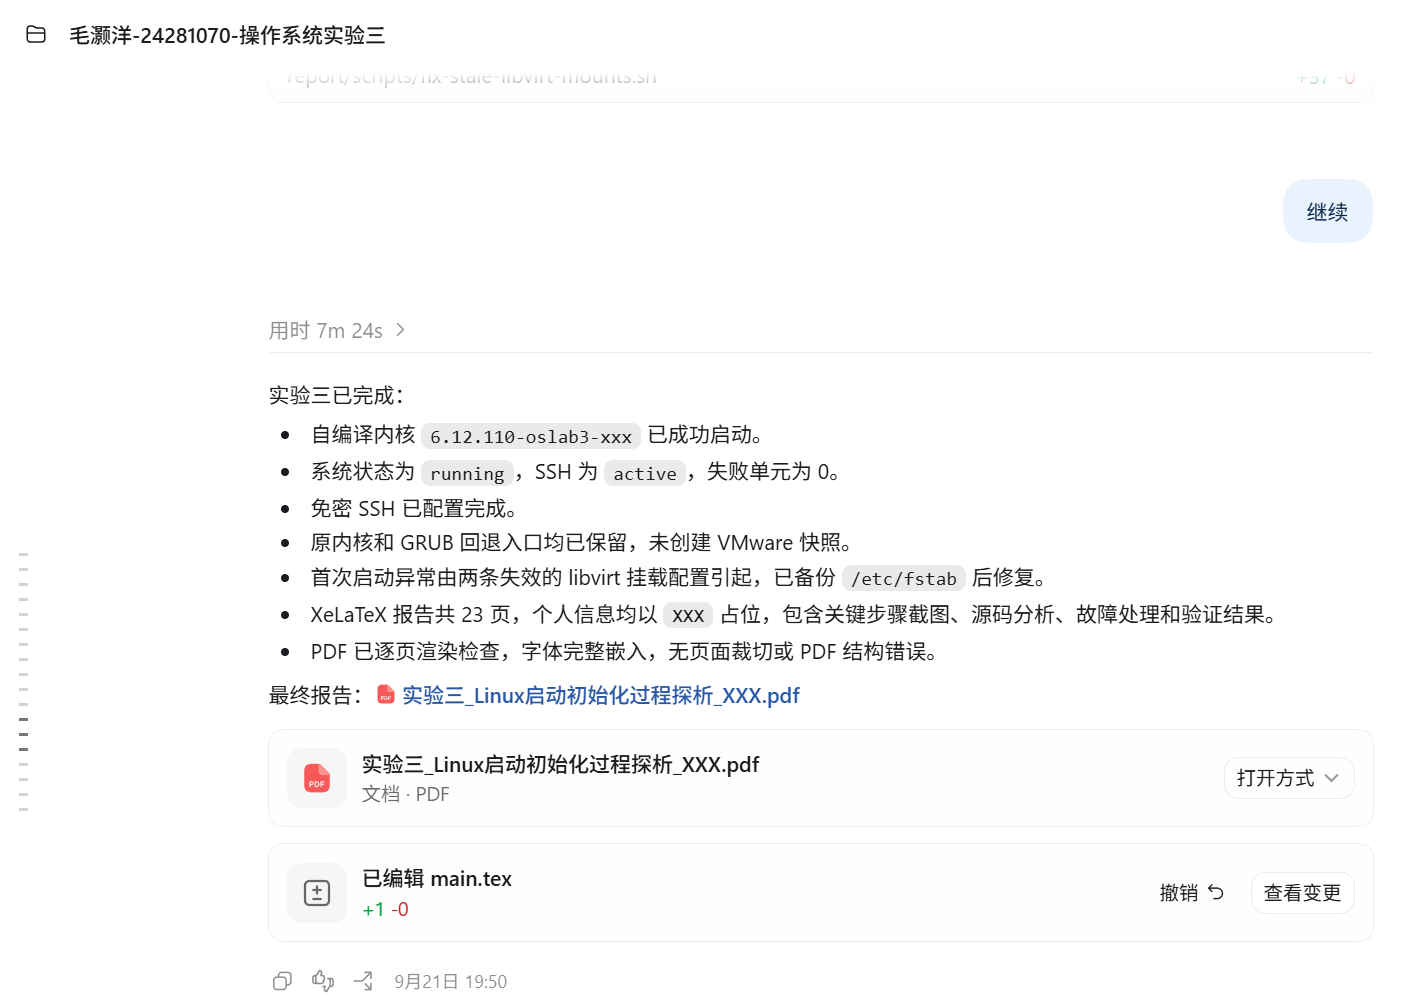
\includegraphics[width=0.96\textwidth]{../ai-record/完成.png}
\caption{个人标题对话截图：基础实验完成反馈（历史版本）}
\end{figure}
其余长截图保留原始分辨率供在仓库放大查阅，不缩成难以辨认的整页插图。
当前公开仓库：\url{https://github.com/oknyhm/os_lab1_3}。仓库名称按用户要求设定，内容仅涵盖实验三。

\chapter{疑难解惑、经验与结论}

\section{疑难解惑}
\begin{description}[style=nextline]
  \item[为什么不能只编译成功而不重启？]
  编译只说明源代码能生成映像，不能证明引导程序、initramfs、根文件系统驱动和用户空间均可用。
  \item[为什么保留旧内核？]
  新配置可能遗漏存储或网络驱动。旧内核提供不依赖 VMware 快照的可恢复路径。
  \item[为什么区分两个 \texttt{startup\_64}？]
  压缩内核与正式内核映像位于不同阶段：前者负责解压和重定位准备，后者进入解压后的内核主体。
  \item[为什么使用唯一版本后缀？]
  可避免与发行版内核混淆，并使 \texttt{uname -r}、模块目录、initramfs 和 GRUB 条目形成一致标识。
\end{description}

\section{四个关键原理问题}
以下解释结合现有实现与日志，由 Agent 协助整理；不是新增实机测试或独立完成声明。
\begin{description}[style=nextline]
\item[进入 emergency mode 是否说明新内核启动失败？]
不一定。它可能出现在内核进入用户空间之后。本次 \texttt{uname -r} 返回新内核版本，
Btrfs 根分区已挂载，说明应继续检查 systemd 挂载和服务，而不能仅凭未进入桌面就判定内核失败。
当时诊断指向失效的 libvirt 挂载配置，修复后系统恢复。
\item[Btrfs 编译成模块，如何挂载 Btrfs 根文件系统？]
引导器同时加载内核和 initramfs，早期用户空间从内存中的 initramfs 加载存储及 Btrfs 模块，
再挂载真正的根文件系统并切换过去。前提是 initramfs 包含匹配版本的模块及依赖；
模块仅安装在尚未挂载的根分区中，并不足以保证启动。
\item[6557 ms 测量的是什么？]
它是模块初始化函数执行时读取的开机相对时间，包含时钟定义中的休眠时间。
没有测量函数结束与开始的差值，因此不是模块执行耗时，也不是
\texttt{start\_kernel()} 或整个启动过程的总耗时。本探针在用户空间服务触发加载时才执行。
\item[为什么早期手动加载也能通过 T05？]
T05 只判断装载时间小于 120000 ms。开机后第 30 秒手动加载同样满足阈值，
所以只能证明较早装载。自动加载结论还要结合配置、真实重启及没有手动加载的过程；
最好同时保留 boot ID、模块加载服务日志和内核日志。
\end{description}

\section{结论与体会}
本实验将 Linux 启动过程从抽象描述落实到具体源码文件、函数入口、配置选项、编译产物和启动日志。
最重要的认识是：启动并非单个函数完成，而是固件、引导器、处理器模式切换、体系结构相关初始化、
通用内核子系统和用户空间 PID 1 逐级交接的过程。配置裁剪用于减少构建范围，未做裁剪前后耗时对照；配置变更必须以实际硬件
和保留原内核为安全边界。基础实验通过两次真实重启、运行版本、Btrfs 根挂载、systemd、网络与 SSH
状态验证源码分析，并区分内核问题与原系统陈旧 fstab 配置。额外设计的启动探针进一步把
\texttt{module\_init()}、procfs、内核日志和 systemd 自动装载连成可运行、可卸载、可测试的闭环；
这一设计提供了观察模块装载与用户空间服务联系的具体入口。运行结果、测试覆盖与个人理解是不同层次，
需要分别用日志、测试断言和本人解释支撑。

\appendix
\chapter{主要命令清单}
\begin{lstlisting}[language=bash]
# 下载与校验
curl -fL -o linux-6.12.110.tar.xz \
  https://cdn.kernel.org/pub/linux/kernel/v6.x/linux-6.12.110.tar.xz
sha256sum linux-6.12.110.tar.xz
tar -xf linux-6.12.110.tar.xz
cd linux-6.12.110

# 配置：先核对实验环境
cp /boot/config-6.11.0-26-kfocus .config
make olddefconfig
yes '' | make localmodconfig
scripts/config --set-str LOCALVERSION '-oslab3-xxx'
scripts/config --disable LOCALVERSION_AUTO
scripts/config --set-str SYSTEM_TRUSTED_KEYS ''
scripts/config --set-str SYSTEM_REVOCATION_KEYS ''
scripts/config --disable DEBUG_INFO_BTF
make syncconfig

# 编译、安装与验证
make -j2
sudo make modules_install
sudo make install
sudo update-grub
sudo reboot
# 在 GRUB 选择目标内核，重连 SSH 后验证
uname -r
journalctl -b -k --no-pager

\end{lstlisting}
\Needspace{19\baselineskip}
以下从本仓库根目录执行，安装需要目标内核及其已完成构建的源码树。新日志使用单独目录。
\begin{lstlisting}[language=bash]
cd extra-design
bash install-probe.sh
sudo reboot
# 重连后重新进入仓库根目录，不要手动加载模块
run_dir="$(mktemp -d /tmp/oslab3-run.XXXXXX)"
set -o pipefail
bash tests/test_boot_probe.sh 2>&1 | tee "$run_dir/probe.log"
test_rc=${PIPESTATUS[0]}
printf 'test_exit=%s\n' "$test_rc" | tee -a "$run_dir/probe.log"
python3 tests/check_probe_contract.py 2>&1 | tee "$run_dir/contract.log"
test_rc=${PIPESTATUS[0]}
printf 'test_exit=%s\n' "$test_rc" | tee -a "$run_dir/contract.log"
bash tests/collect-boot-performance.sh "$run_dir"
\end{lstlisting}

\chapter{实验文件与日志}
\begingroup\small
\begin{longtable}{p{0.54\textwidth}p{0.38\textwidth}}
  \toprule
  文件 & 内容 \\
  \midrule
  \path{report/main.tex} & 本报告 XeLaTeX 源文件 \\
  \path{report/figures/} & 原始实验截图 \\
  \path{report/logs/environment.txt} & 实验环境完整记录 \\
  \path{report/logs/configuration.log} & 配置转换日志 \\
  \path{report/logs/source-index.txt} & 关键源码入口与行号 \\
  \path{report/logs/build.log} & 内核编译完整输出 \\
  \path{report/logs/build-attempt1.log} & 首轮 BTF 链接失败日志 \\
  \path{report/logs/build.status} & 成功构建状态与结束时间 \\
  \path{report/logs/install.log} & 模块、内核、initramfs 与 GRUB 安装日志 \\
  \path{report/logs/kernel-config-6.12.110-oslab3-xxx} & 最终内核配置 \\
  \path{report/logs/fstab-backup.txt} & fstab 备份路径及 SHA-256 \\
  \path{report/logs/boot-verification.txt} & 新内核启动验证结果 \\
  \path{extra-design/oslab3_probe.c} & 启动探针内核模块源码 \\
  \path{extra-design/oslab3_probe.conf} & systemd 模块自动加载配置 \\
  \path{tests/test_boot_probe.sh} & 九项自动化验证脚本 \\
  \path{report/logs/extra-design-install.log} & 模块编译与安装记录 \\
  \path{report/logs/extra-design-manual-test.log} & 手动加载、卸载和日志记录 \\
  \path{report/logs/extra-design-test.log} & 重启后九项 PASS 结果 \\
  \path{report/logs/boot-performance.txt} & 启动耗时、服务排序和关键链 \\
  \path{report/figures/boot-analysis.svg} & systemd 启动时序原始图 \\
    \path{ai-record/README.md} & Agent 对话证据选择与脱敏说明 \\
    \path{ai-record/dialogue-excerpts.md} & 当前会话的脱敏文字节选（非完整导出） \\
    \path{docs/test-matrix.md} & 功能、测试结果和证据边界 \\
    \path{tests/check_probe_contract.py} & 补充接口检查与夹具自测 \\
    \path{report/logs/contract-self-test-20261007.txt} & 本机自测输出，非实机结果 \\
    \path{report/logs/supplemental-vm-20261007.txt} & 10 月 7 日实机补测完整记录 \\
    \path{report/scripts/run-supplemental-verification.sh} & 补测命令及退出码采集脚本 \\
  \bottomrule
\end{longtable}

\endgroup
\begin{thebibliography}{9}
  \addcontentsline{toc}{chapter}{参考文献}
  \bibitem{kernelreleases}
  The Linux Kernel Archives. \emph{Active kernel releases}.\\
  \url{https://www.kernel.org/}

  \bibitem{kernelsource}
  The Linux Kernel Archives. \emph{Linux 6.12.110 source archive}.\\
  \url{https://cdn.kernel.org/pub/linux/kernel/v6.x/linux-6.12.110.tar.xz}

  \bibitem{kernelboot}
  Linux kernel documentation. \emph{x86 Boot Protocol}.\\
  \url{https://docs.kernel.org/arch/x86/boot.html}

  \bibitem{kernelbuild}
  Linux kernel documentation. \emph{Kbuild}.\\
  \url{https://docs.kernel.org/kbuild/}

  \bibitem{guide}
  翟高寿. \emph{操作系统实验指导：Linux 启动初始化过程探析}. 北京交通大学计算机学院, 2022.
\end{thebibliography}

\end{document}
